The Motor Control Layer controls the machine frame and executes actions requested by the core logic layer. The commands will be sent through a serial interface in the G-Code syntax. The Motor Control Layer will parse these commands, translate them to the machine required machine configuration, and manipulate the motors on the frame to match. If the commands are sensor data requests the I/O handler will translate the raw sensor data into a string format and transmit it back across the serial interface.

\begin{figure}[h!]
	\centering
 	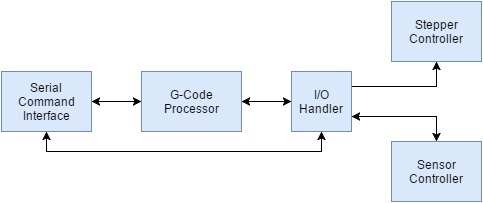
\includegraphics[width=0.60\textwidth]{images/motor_control_layer}
 \caption{Example subsystem description diagram}
\end{figure}

\subsection{Serial Command Interface}
Ther Serial Command Interface is the only method of communication available to the entire Motor Control Layer. This subsystem receives character input through a serial bus and must parse them into individual instructions. These instructions are then routed to the appropriate subsystem for execution. The interface will also build return statements and transmit them as requested by the other Motor Control Layer subsystems. 

\subsubsection{Assumptions}
The Serial Command Interface should not receive commands longer than the limiting buffer. Any commands which are longer than that will not be executed, returning an error through the Serial Command Interface to the control system. The control system is assumed to understand that a command was unable to be parsed and attempt to recover without further action from the Serial Command Interface.

\subsubsection{Responsibilities}
The Serial Command Interface is responsible for parsing all character input into parametrized commands for consumption by the appropriate subsystem. The interface must request a retransmit if there is an error in parsing the input or return a command acknowledged message if parsing was successful. When the Serial Control Interface sends a message to the Core Logic Layer it does not expect a result. 

\subsubsection{Subsystem Interfaces}

\begin {table}[H]
\caption {Subsystem interfaces} 
\begin{center}
    \begin{tabular}{ | p{1cm} | p{6cm} | p{3cm} | p{3cm} |}
    \hline
    ID & Description & Inputs & Outputs \\ \hline
    \#01 & Serial Bus Interface & \pbox{3cm}{characters over bus} & \pbox{3cm}{characters over bus}  \\ \hline
    \end{tabular}
\end{center}
\end{table}

\subsection{G-Code Processor}
The G-Code Processor processes Cartesian coordinate commands into polar configurations which can be used to control the machine. 

\subsubsection{Responsibilities}
This subsystem must intercept control commands which were sent using Cartesian coordinates and convert them to polar coordinates before passing them to the I/O Handler subsystem.  

\subsubsection{Subsystem Interfaces}

\begin {table}[H]
\caption {Subsystem interfaces} 
\begin{center}
    \begin{tabular}{ | p{1cm} | p{6cm} | p{3cm} | p{3cm} |}
    \hline
    ID & Description & Inputs & Outputs \\ \hline
    \#01 & Serial Command Interface & \pbox{3cm}{String array} & \pbox{3cm}{N/A}  \\ \hline
    \#02 & I/O Handler & \pbox{3cm}{N/A} & \pbox{3cm}{String array}  \\ \hline
    \end{tabular}
\end{center}
\end{table}

\subsection{I/O Handler}
The I/O Handler executes motor control as requested by the Serial Command Interface and the G-Code Processor. These commands are received as an array of strings. The I/O Handler calculates the required motor actions to bring the machine into the desired state and passes the actions to the Motor Control Layer. If the Serial Command Interface requests sensor data, the I/O Handler will parse the raw data into an established format to send back through the Serial Command Interface.

\subsubsection{Assumptions}
The I/O Handler should never have to parse unknown sensor data. 

\subsubsection{Responsibilities}
The I/O Handler must maintain an internal store of machine state and be able to execute some default motor action to detect and establish machine state.

\subsubsection{Subsystem Interfaces}
\begin {table}[H]
\caption {Subsystem interfaces} 
\begin{center}
    \begin{tabular}{ | p{1cm} | p{6cm} | p{3cm} | p{3cm} |}
    \hline
    ID & Description & Inputs & Outputs \\ \hline
    \#01 & Stepper Controller & \pbox{3cm}{Number of steps required} & \pbox{3cm}{N/A}  \\ \hline
    \#02 & Sensor Controller & \pbox{3cm}{N/A} & \pbox{3cm}{Raw Sensor Data}  \\ \hline
    \end{tabular}
\end{center}
\end{table}

\subsection{Motor Control}
The Motor Control subsystem is the primary driver for the motors on the FarmBot. It will execute motion commands as requested by the I/O Handler subsystem. 

\subsubsection{Assumptions}
The I/O Handler may request actions from the Motor Control system which would be harmful to the machine. The Motor Control system should prioritize safe operation over faithful command execution. 

\subsubsection{Responsibilities}
The Motor Control subsystem should execute commands given to it in the expected format. 

\subsubsection{Subsystem Interfaces}
\begin {table}[H]
\caption {Subsystem interfaces} 
\begin{center}
    \begin{tabular}{ | p{1cm} | p{6cm} | p{3cm} | p{3cm} |}
    \hline
    ID & Description & Inputs & Outputs \\ \hline
    \#01 & I/O Handler interface & \pbox{3cm}{Commands} & \pbox{3cm}{N/A}  \\ \hline
    \#02 & Stepper Motor Driver & \pbox{3cm}{N/A} & \pbox{3cm}{step \\ direction}  \\ \hline
    \end{tabular}
\end{center}
\end{table}

\subsection{Sensor Control}
The Sensor Control subsystem allows easier interfacing with sensor systems.

\subsubsection{Assumptions}
All sensors will be configured for input parsing in the Sensor Control subsystem. 

\subsubsection{Responsibilities}
The Sensor Control system will only be responsible for unifying and normalizing sensor input data.

\subsubsection{Subsystem Interfaces}
\begin {table}[H]
\caption {Subsystem interfaces} 
\begin{center}
    \begin{tabular}{ | p{1cm} | p{6cm} | p{3cm} | p{3cm} |}
    \hline
    ID & Description & Inputs & Outputs \\ \hline
    \#01 & I/O Handler Interface \pbox{3cm}{Sensor Requests \\ Sensor Configuration} & \pbox{3cm}{Sensor Data}  \\ \hline
    \#02 & Sensors & \pbox{3cm}{Sensor Configuration} & \pbox{3cm}{Sensor Data}  \\ \hline
    \end{tabular}
\end{center}
\end{table}
